As a systems research project, the focus of this study revolves around software and, in particular, developing more efficient data-intensive computing pipelines that find wide applications in \gls{ML} and the training of neural networks. Software, according to the Green Software Foundation \footnote{Foundation's website available at \url{https://greensoftware.foundation/}}, can be "part of the climate problem or part of the climate solution" \cite{WhatGreenSoftware2021}. Green Software can be defined as software that reduces its environmental impact by using less physical resources and less energy and optimizing energy use to use lower-carbon sources \cite{WhatGreenSoftware2021}. In the context of \gls{ML} and training of neural networks, reducing training time (and so also the read and write latency operation on the dataset) has been proven to positively impact the reduction in carbon emissions~\cite{pattersonCarbonEmissionsLarge2021,pattersonCarbonFootprintMachine2022}.

This project contributes to the \glspl{SDG}~\footnote{\glspl{SDG} website available at \url{https://sdgs.un.org/}} 7~--~Affordable and Clean Energy and 9~--~Industry Innovation and Infrastructure, more specifically the targets 7.3~--~Double the improvement in energy efficiency and 9.4~--~Upgrade all industries and infrastructures for sustainability. This thesis contributes to these goals by reducing latency and thus increasing the data throughput for reading and writing on Delta Lake tables on \gls{HopsFS}. This purpose also follows the fundamental green software principles reducing \gls{CPU} time use compared to the previous system. Reducing \gls{CPU} usage time reduces energy consumption, leading to a lower carbon footprint.

\begin{figure}
    \centering
    \begin{subfigure}[b]{0.5\linewidth}
        \centering
        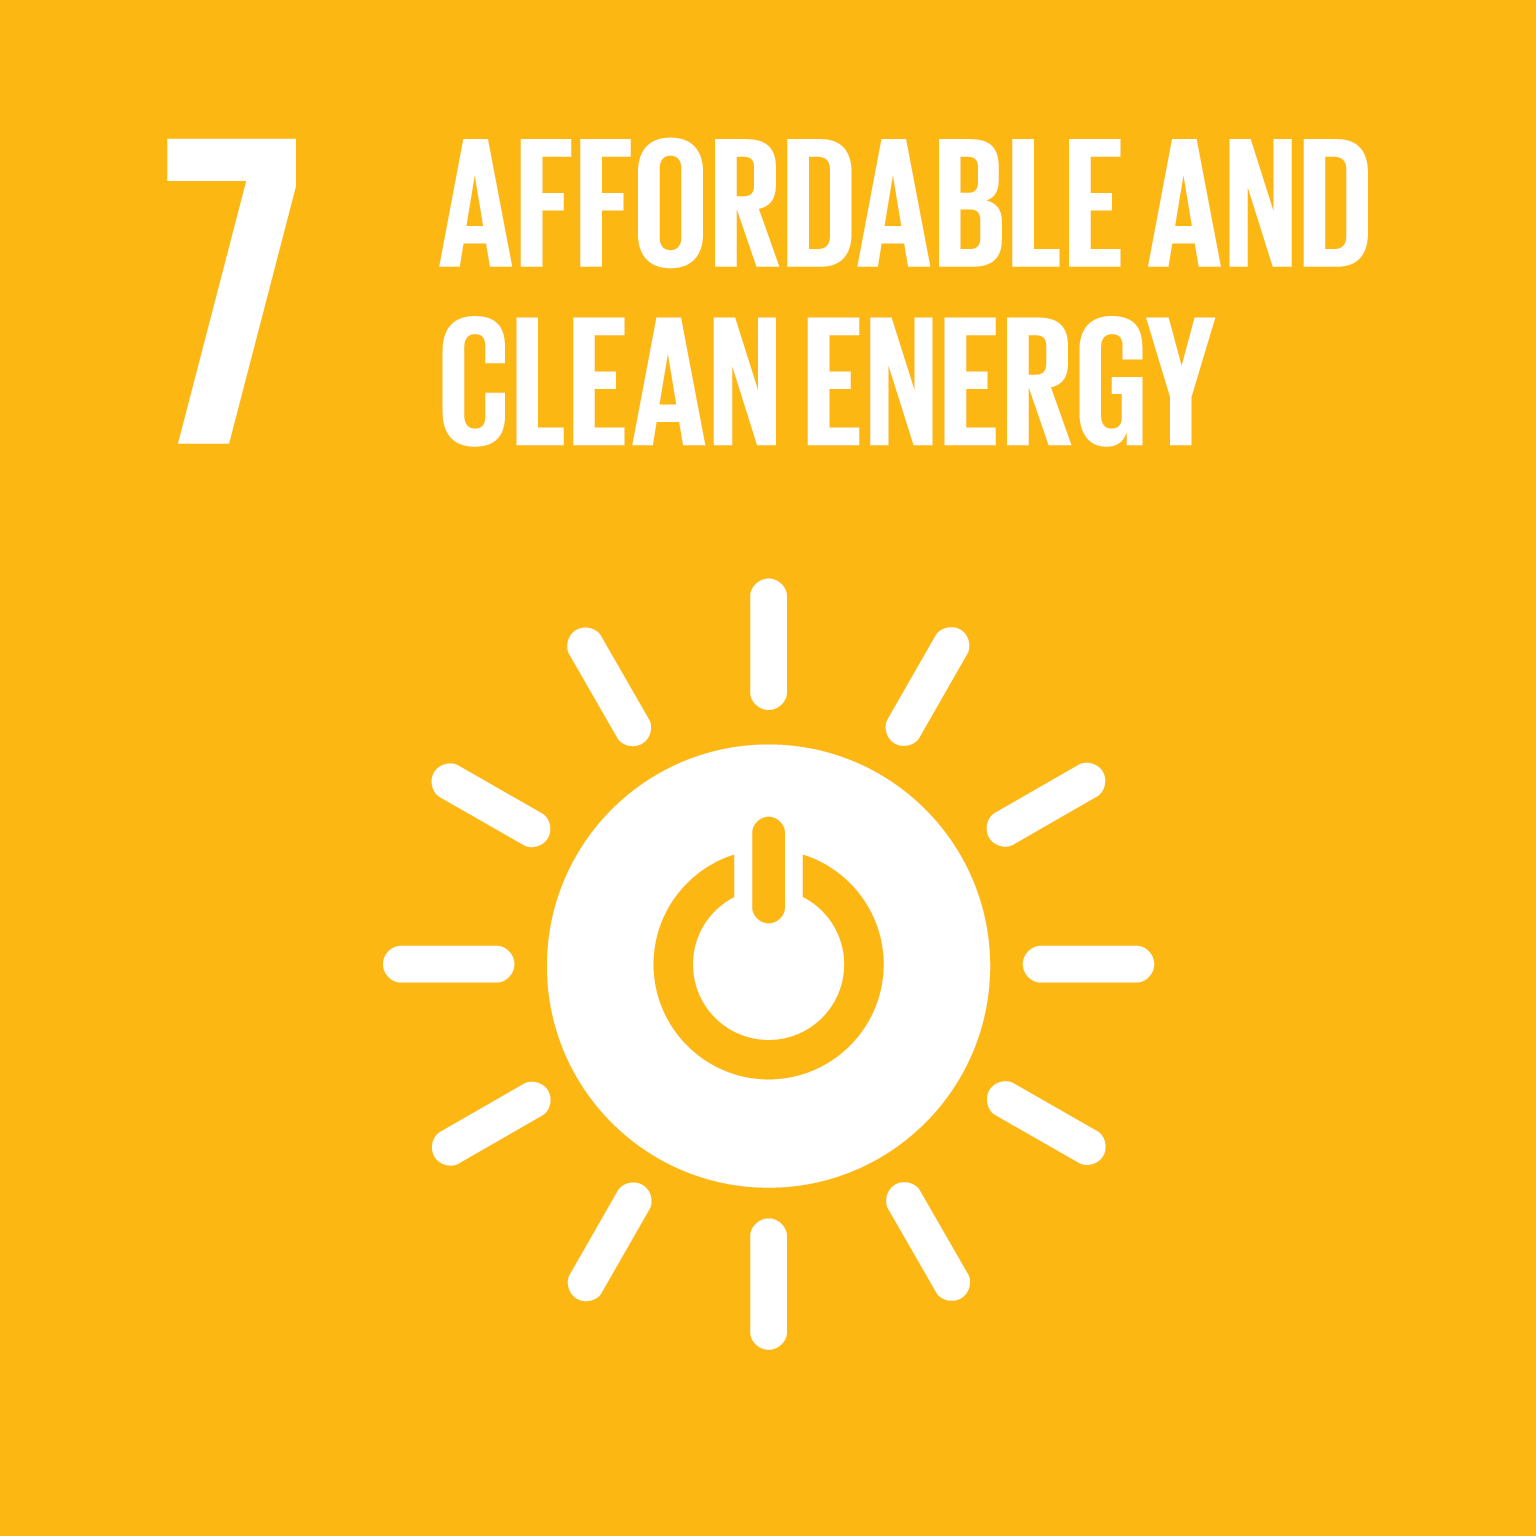
\includegraphics[width=0.6\linewidth]{figures/1-introduction/E_SDG_goals_icons-07.png} 
        \label{fig:sdg07}
    \end{subfigure}\hfill
    \begin{subfigure}[b]{0.5\linewidth}
        \centering
        
\includegraphics[width=0.6\linewidth]{figures/1-introduction/E_SDG-goals_icons-09.png}
        \label{fig:sdg09}
	\end{subfigure}
	\caption[Sustainable Development Goals supported by this thesis]{Illustrations of the \glstext{SDG} supported by this thesis.}
	\label{fig:sdgs}
\end{figure}

Ultimately, this will lead to improved energy efficiency and reduced carbon footprint of data-intensive computing pipelines, which find wide applications in \gls{ML} and neural network training.
